
%%%%%%%%%%%%%%%%%%%%%%%%%%%%%%%%%%%%%%%%%%%%%%%%%%%%%%%%%%%%%%%%%%%%%%%%%%%%%%%%%%%%%%%
%%%%%%%%%%%%%%%%%%%%%%%%%%%%%%%%%%%%%%%%%%%%%%%%%%%%%%%%%%%%%%%%%%%%%%%%%%%%%%%%%%%%%%%
% 
% This top part of the document is called the 'preamble'.  Modify it with caution!
%
% The real document starts below where it says 'The main document starts here'.

\documentclass[12pt]{article}

\usepackage{amssymb,amsmath,amsthm}
\usepackage[top=1in, bottom=1in, left=1.25in, right=1.25in]{geometry}
\usepackage{fancyhdr}
\usepackage{enumerate}
\usepackage{listings}
\usepackage{graphicx}
\usepackage{float}
\usepackage{multicol}
% Comment the following line to use TeX's default font of Computer Modern.
\usepackage{times,txfonts}
\usepackage{mwe}
\usepackage{caption}
\usepackage{subcaption}
\usepackage{svg}





\makeatletter
\renewcommand*\env@matrix[1][*\c@MaxMatrixCols c]{%
  \hskip -\arraycolsep
  \let\@ifnextchar\new@ifnextchar
  \array{#1}}
\makeatother

\newtheoremstyle{homework}% name of the style to be used
  {18pt}% measure of space to leave above the theorem. E.g.: 3pt
  {12pt}% measure of space to leave below the theorem. E.g.: 3pt
  {}% name of font to use in the body of the theorem
  {}% measure of space to indent
  {\bfseries}% name of head font
  {:}% punctuation between head and body
  {2ex}% space after theorem head; " " = normal interword space
  {}% Manually specify head
\theoremstyle{homework} 

% Set up an Exercise environment and a Solution label.
\newtheorem*{exercisecore}{Exercise \@currentlabel}
\newenvironment{exercise}[1]
{\def\@currentlabel{#1}\exercisecore}
{\endexercisecore}

\newcommand{\localhead}[1]{\par\smallskip\noindent\textbf{#1}\nobreak\\}%
\newcommand\solution{\localhead{Solution:}}

%%%%%%%%%%%%%%%%%%%%%%%%%%%%%%%%%%%%%%%%%%%%%%%%%%%%%%%%%%%%%%%%%%%%%%%%
%
% Stuff for getting the name/document date/title across the header
\makeatletter
\RequirePackage{fancyhdr}
\pagestyle{fancy}
\fancyfoot[C]{\ifnum \value{page} > 1\relax\thepage\fi}
\fancyhead[L]{\ifx\@doclabel\@empty\else\@doclabel\fi}
\fancyhead[C]{\ifx\@docdate\@empty\else\@docdate\fi}
\fancyhead[R]{\ifx\@docauthor\@empty\else\@docauthor\fi}
\headheight 15pt

\def\doclabel#1{\gdef\@doclabel{#1}}
\doclabel{Use {\tt\textbackslash doclabel\{MY LABEL\}}.}
\def\docdate#1{\gdef\@docdate{#1}}
\docdate{Use {\tt\textbackslash docdate\{MY DATE\}}.}
\def\docauthor#1{\gdef\@docauthor{#1}}
\docauthor{Use {\tt\textbackslash docauthor\{MY NAME\}}.}
\makeatother



\usepackage{mathabx}





% Shortcuts for blackboard bold number sets (reals, integers, etc.)
\newcommand{\Reals}{\ensuremath{\mathbb R}}
\newcommand{\Nats}{\ensuremath{\mathbb N}}
\newcommand{\Ints}{\ensuremath{\mathbb Z}}
\newcommand{\Rats}{\ensuremath{\mathbb Q}}
\newcommand{\Cplx}{\ensuremath{\mathbb C}}
%% Some equivalents that some people may prefer.
\let\RR\Reals
\let\NN\Nats
\let\II\Ints
\let\CC\Cplx

%%%%%%%%%%%%%%%%%%%%%%%%%%%%%%%%%%%%%%%%%%%%%%%%%%%%%%%%%%%%%%%%%%%%%%%%%%%%%%%%%%%%%%%
%%%%%%%%%%%%%%%%%%%%%%%%%%%%%%%%%%%%%%%%%%%%%%%%%%%%%%%%%%%%%%%%%%%%%%%%%%%%%%%%%%%%%%%
% 
% The main document start here.

% The following commands set up the material that appears in the header.
\doclabel{Math 614: Homework 9}
\docauthor{Stefano Fochesatto}
\docdate{\today}

\begin{document}


\begin{exercise}{P22} Consider the graph of five web pages a, b, c, d, e, shown below, where each page links to some of the other pages as show. The goal 
  of this problem, is to compute the Google PageRank of the pages. In fact, this problem, is about the essential idea which 
  created Google, only about 25 years ago. 
  \begin{figure}[H]
    \begin{center}
      \caption{P22 graph}
       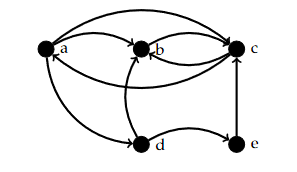
\includegraphics[width=.5\textwidth]{fig1.png}
    \end{center}
  \end{figure}
\begin{enumerate}
  \item[a.] Start by asking Google to document itself. Go to Google Scholar and search for 'pagerank citation ranking'.The first link,  the one with highest PageRank,  will 
  be a technical preprint by Page, Brin, Motwani, and Winograd;  it has more than 15000 citations. Download the 17 page PDF and read it. It describes a simpler time. 
  
  The main ideas are about a 
  web as a directed graph, as in the example shown above, that the limiting probability that a certain random web surfer visits any particular page is its PageRank, and finally that a 
  search engine should report results in the Page Rank order. We can regard PageRank as simply an eigenvector of a certain matrix $A$, a transition probability matrix for a Markov chain. To 
  build $A$ we will start with the adjacency matrix $G$ of the web. Here is how to start with a web as directed graph and construct $G$,$A$ and the eigenvector of PageRank values: \\
  Let $W$ be a connected directed graph of $n$ webpages, index the pages 1 through n. Let $G$, be the $nxn$ connectivity matrix $W$ that is, 
  \begin{equation*}
    g_{ij} = 
    \left\{
      \begin{array}{ll}
            1 & \text{There is a hyperlink to $i$ from $j$} \\
            0 & \text{Otherwise} \\
      \end{array} 
      \right\}
  \end{equation*}

  The number of nonzeros in $G$ is the total number of hyperlinks in $W$. Let $c_j$ be the columns sums of $G$;
  \begin{equation*}
    c_j = \sum_{i = 1}^n g_{ij}
  \end{equation*}

The value of $c_j$ gives the outdegreee of the $jth$ page. Let $p$ be the fraction of the time that the random walk follows some link, 
so $1-p$ is the fraction of time that an arbitrary page is chose. Define $\delta = (1 - p)/n$.Now let $A$ be the $nxn$
 matrix whose entries are, 
 \begin{equation*}
   a_{ij} = \dfrac{pg_{ij}}{c_{j}} + \delta
 \end{equation*}
 The matrix $A$ is the transition probability matrix of the random-surfer Markov chain. An old theorem says the largest eigenvalue of $A$ is equal to one
 and the corresponding eigenvector $x$, which satisfies
 \begin{equation*}
   Ax = x
 \end{equation*}
 is unique up to a scaling factor, and has positive entries. Choose the scaling so that,
 \begin{equation*}
   1 = \sum_{i = 1}^n x_i.
 \end{equation*}
 The entries of $x$ are the Page Ranks of webpages in $W$.\\
 For a realistic web, $G$ is huge and sparse because most pairs of webpages are not connected by a single link. Google suggests $p = .85$.
 Matrix $A$ is not spare because most entries are equal to the small constant $\delta > 0$. The 'old' Perron-Frobenius Theorem says that if all entries in a matrix
 are positive then all the entries of the eigenvector associated to the largest eigenvalue can we chose to be positive.\\


 \vspace{1in}

 \item[b.] Folling my description of the process, compute $G$ for the web shown above. \\
 \solution From the passage above we know that $G$ is the adjacency matrix for the figure 1. Building the adjacency matrix we get, 
 \begin{equation*}
   \begin{bmatrix}
     0 & 0 & 1 & 0 & 0\\
     1 & 0 & 1 & 1 & 0\\
     1 & 1 & 0 & 0 & 1\\
     1 & 0 & 0 & 0 & 0\\ 
     0 & 0 & 0 & 1 & 0
   \end{bmatrix}
 \end{equation*}
 \vspace{1in}


 \item[c.] Continuing from my description, build $A$ from $G$ using $p = .85$ as suggested. 
 Finally, use Matlabs eig() to compute the PageRanks. Which page gets the highest PageRank?
 explain in intuitive terms.\\
 \solution The following Matlab script computes $A$ from $G$, and uses the eig() function to compute the PageRanks.\\
 \\
 \textbf{Code:}
 \begin{center}
   \lstinputlisting[basicstyle = \small]{P22C.m}
 \end{center} 
 \textbf{Console:}
 \begin{center}
   \lstinputlisting[basicstyle = \small]{P22C.txt}
 \end{center} 
 From our results we can see that pages sorted by PageRank are $c, b, a, d, e$. C is likely rated the highest since it shares a loop with 
 the next two highest pages $a$ and $b$ in terms of total degree. It also makes sense that $b$ is second highest as it has the same in-degree as 
 $c$ except they are from pages with lesser total degree.  
 \vspace{1in}


 \item[d.] Draw a new web $W$ with 10 pages. Recompute $G$, $A$, and the PageRanks.\\
 \solution The following Matlab script generates a 10 node directed graph(web) $W$ by generating $G$ and computes $A$, and 
 the PageRanks.\\
 \\
 \begin{figure}[H]
  \begin{center}
    \caption{Generated P22D graph}
     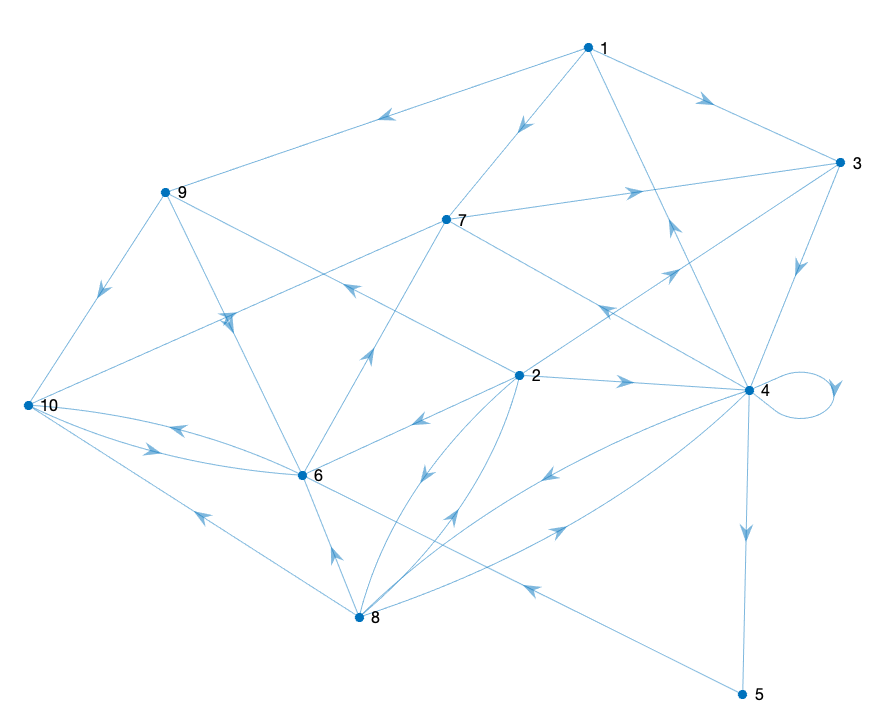
\includegraphics[width=.8\textwidth]{P22DGraph.png}
  \end{center}
\end{figure}
 \textbf{Code:}
 \begin{center}
   \lstinputlisting[basicstyle = \small]{P22D.m}
 \end{center} 
 \textbf{Console:}
 \begin{center}
   \lstinputlisting[basicstyle = \tiny]{P22D.txt}
 \end{center} 


\item[ExtraCredit] Build a random wlak probram which traverses a web as would a Google 'bot'.
Build-up an estimate of PageRank based in the fraction of the time spent at a given page. It is up to 
you how to represent a web in some data structure; it could be the matrix $G$, or not. Check that your surfer converges to the results computed in 
parts $c$ and $d$.\\
\solution Consider the following code, \\
\textbf{Code:}
\begin{center}
  \lstinputlisting[basicstyle = \small]{RandomWalk.m}
\end{center} 
\textbf{Console:}
\begin{center}
  \lstinputlisting[basicstyle = \tiny]{ExtraCredit.txt}
\end{center} 












\end{enumerate}
\end{exercise}





\vspace{1in}

\begin{exercise}{20.1} Let $A \in \CC^{mxm}$ be nonsingular. Show that $A$ has an LU factorization if and only if for each $k$ with 
  $1 \leq k \leq m$, the upper-left $kxk$ block of $A_{1:k, 1:k}$ is nonsingular.(Hint: The row operations of Gaussian elimination leave the 
  determinants of $A_{1:k, 1:k}$ unchanged.) Prove that this LU factorization is unique. \\
  \begin{proof} Suppose that $A \in \CC^{mxm}$ is nonsingular and that has an LU factorization. Recall that term-wise each $a_{ij}$ is produced by the 
    following inner-products, 
    \begin{equation*}
      a_{ij} = L_i^*U_j
    \end{equation*}
    where $L_i$ is the ith row of $L$ and $U_j$ is the jth column of $U$. Since $L$ and $U$ are triangular for $i, j \leq k$, since it only removes the addition of zeros,  
    \begin{equation*}
      a_{ij} = L_i^*U_j = L_{i[1:k, 1:k]}, ^*U_{j[1:k, 1:k]}. 
    \end{equation*} 
    Analogously it follows that, 
    \begin{equation*}
      A_{1:k, 1:k} = L_{1:k, 1:k}U_{1:k, 1:k}. 
    \end{equation*}
    Therefore each upper-left $kxk$ block of $A_{1:k, 1:k}$ has an LU factorization. Consider taking the determinant of both sides of the previous equation, and let $u$ be terms in $U$, 
    \begin{align*}
     det(A_{1:k, 1:k}) &= det(L_{1:k, 1:k}U_{1:k, 1:k}),\\
     det(A_{1:k, 1:k}) &= det(L_{1:k, 1:k}) det(U_{1:k, 1:k}),\\
     det(A_{1:k, 1:k}) &= 1 \prod_{i = 1}^m u_{i, i}.
    \end{align*} 
    Since $A$ is nonsingular with a full LU factorization we know that none of the terms in the diagonal of $U$ can be zero and therefore $det(A_{1:k, 1:k}) \neq 0$.\\


    \vspace{1in}
    Suppose that $A \in \CC^{mxm}$ be nonsingular and for each $k$ with 
    $1 \leq k \leq m$, the upper-left $kxk$ block of $A_{1:k, 1:k}$ is nonsingular. To prove that $A$ has an LU factorization we will proceed by induction on $k$.
    The base case is clearly true, 
    \begin{align*}
      A_{1, 1} &= 1*a_1.\\
       &=  L_{1, 1}U_{1, 1},
    \end{align*}
    Which must be valid since $A_{1, 1}$ is nonsingular. Suppose that there exist an LU factorization for some $A_{k, k}$. Now consider $A_{k+1, k+1}$ and note it's relation to $A_{k, k}$.
     As an aside we should note that for all dimensions of $A$ we are bounded above by $m$. Let $\hat{v}, d$ and $\hat{u}, d$ be the final row and column of $A_{k+1, k+1}$ respectively, 
    \begin{equation*}
      A_{k+1, k+1} = 
      \begin{bmatrix}
        A_{k, k} & \hat{u}\\
        \hat{v} & d
      \end{bmatrix}
    \end{equation*}
    Recall that by the induction hypothesis, $A_{k, k}$ has an LU factorization so there must exist some factor such that, 
    \begin{equation*} 
      \begin{bmatrix}
        L_{k, k} & 0\\
        \hat{v}U^{-1}_{k, k} & 1
      \end{bmatrix}
      \begin{bmatrix}
        U_{k, k} & L^{-1}_{k, k}\hat{u}\\
        0 & -\hat{v}U^{-1}_{k, k}L^{-1}_{k, k}\hat{u} + d
      \end{bmatrix} = 
      \begin{bmatrix}
        L_{k, k}U_{k, k} + 0 & L_{k, k}L^{-1}_{k, k}\hat{u} + 0\\
        \hat{v}U^{-1}_{k, k}U_{k, k} + 0 & \hat{v}U^{-1}_{k, k}L^{-1}_{k, k}\hat{u}-\hat{v}U^{-1}_{k, k}L^{-1}_{k, k}\hat{u} + d
      \end{bmatrix} = 
      \begin{bmatrix}
        A_{k, k} & \hat{u}\\
        \hat{v} & d
      \end{bmatrix} 
    \end{equation*}
    Note that by this factorization $det(A_{k+1, k+1}) = det(U_{k, k})(-\hat{v}U^{-1}_{k, k}L^{-1}_{k, k}\hat{u} + d)$ and since we know that $det(A_{k+1, k+1})$ and $det(U_{k, k})$ are not equal to zero 
    it must be the case that $(-\hat{v}U^{-1}_{k, k}L^{-1}_{k, k}\hat{u} + d)$ is also greater than zero. Thus $A_{k+1, k+1}$ has a valid LU factorization.\\
    
    
    \vspace{1in}
    Suppose that the matrix $A$ has two valid LU factorization $L_1U_1$ and $L_2U_2$. Consider the following matrix algebra, 
    \begin{align*}
      L_1U_1 &= L_2U_2,\\
      L^{-1}_2L_1 &= U_2U^{-1}_1.
    \end{align*}
    Recall that in homework 1 we proved that the inverse of a triangular matrix is also triangular, and clearly the product of two triangular matrices is also triangular. Therefore the last equality shows an 
    upper triangular matrix is equal to a lower triangular matrix, a condition only satisfied by the identity, 
    \begin{equation*}
      L^{-1}_2L_1 = I = U_2U^{-1}_1.
    \end{equation*}
    Thus we get the following equalities  $L_2 = L_1 $ and $U_2 = U_1 $.
  \end{proof}
\end{exercise}


\vspace{1in}



\begin{exercise}{20.1(a)}Suppose an $mxm$ matrix $A$ is written in the block form 
  \begin{equation*}
    A = \begin{bmatrix}
      A_{11} & A_{12}\\
      A_{21} & A_{22}
    \end{bmatrix}
  \end{equation*}
  where $A_{11}$ is an $nxn$ matrix and $A_{22}$ is $(m-n)x(m-n)$ Assume $A$ satisfies the condition in Exercise 20.1. Verify the following, 
  \begin{equation*}
    \begin{bmatrix}
      I & 0 \\
      -A_{21}A^{-1}_{11} & I
    \end{bmatrix}
    \begin{bmatrix}
      A_{11} & A_{12}\\
      A_{21} & A_{22}
    \end{bmatrix}
     = 
     \begin{bmatrix}
       A_{11} & A_{12}\\
       0 & A_{22} - A_{21}A^{-1}_{11}A_{12}
     \end{bmatrix}
  \end{equation*}
  \solution Let's consider each block matrix multiplication individually to ensure that the partition dimension sizes agree for block multiplication. The first multiplication 
  works since the $I$ on the top left must be $nxn$ since $-A_{21}A^{-1}_{11}$ is an $(m - n)xn$ matrix. 
  \begin{equation*}
    IA_{11} + 0 = A_{11}
  \end{equation*}
  Here the dimensions agree since  $-A_{21}$ is an $(m - n)xn$ matrix and  $A^{-1}_{11}$ is an $nxn$ matrix. 
  \begin{equation*}
    -A_{21}A^{-1}_{11}A_{11} + IA_{21} = 0
  \end{equation*}
  This multiplication works since the bottom right $I$ must be an $(m-n)x(m-n)$ identity since $-A_{21}A^{-1}_{11}$ is an $(m - n)xn$ matrix. 
  \begin{equation*}
    IA_{12} + 0 = A_{12}
  \end{equation*}
  Here note that $A_{21}$ is $(m - n)xn$ and $A_{12}$ is $nx(m - n)$ so the product on the right is $(mxm)$. 
  \begin{equation*}
    -A_{21}A^{-1}_{11}A_{12} + A_{22} = A_{22}-A_{21}A^{-1}_{11}A_{12}
  \end{equation*}
\end{exercise}



\vspace{1in}









\begin{exercise}{21.1} Let $A$ be the following $4x4$ matrix, 
  \begin{equation*}
    A = 
    \begin{bmatrix}
      2& 1 &1 &0\\ 
      4& 3 &3 &1\\
      8& 7 &9 &5\\
      6& 7 &9 &8
    \end{bmatrix}
  \end{equation*} 
  \begin{enumerate}
    \item[a] Determine the $det(A)$ using the factorization in (20.5), 
    \begin{equation*}
      \begin{bmatrix}
        2& 1 &1 &0\\ 
        4& 3 &3 &1\\
        8& 7 &9 &5\\
        6& 7 &9 &8
      \end{bmatrix}
       = 
       \begin{bmatrix}
         1&0&0&0\\
         2& 1&0 &0\\
         4& 3& 1&0\\
         3& 4& 1& 1
       \end{bmatrix}
       \begin{bmatrix}
         2 &1 &1& 0\\
         0 &1 &1& 1 \\
         0 &0 &2& 2 \\
         0 &0 &0& 2
       \end{bmatrix}.
    \end{equation*} 
    \solution Using this factorization we can quickly compute the determinant since, the determinant of a triangular matrix is the product of it's diagonal entries. Doing so we get the following, 
    \begin{align*}
      det(A) &= det\left( \begin{bmatrix}
        1&0&0&0\\
        2& 1&0 &0\\
        4& 3& 1&0\\
        3& 4& 1& 1
      \end{bmatrix}
      \begin{bmatrix}
        2 &1 &1& 0\\
        0 &1 &1& 1 \\
        0 &0 &2& 2 \\
        0 &0 &0& 2
      \end{bmatrix}\right),\\
      &=
      det\left(
      \begin{bmatrix}
        1&0&0&0\\
        2& 1&0 &0\\
        4& 3& 1&0\\
        3& 4& 1& 1
      \end{bmatrix}
      \right)
      det\left(
      \begin{bmatrix}
        2 &1 &1& 0\\
        0 &1 &1& 1 \\
        0 &0 &2& 2 \\
        0 &0 &0& 2
      \end{bmatrix}
      \right),\\
      &= 1^2 * 2^3 = 8. 
    \end{align*}
    \vspace{.15in}


    \item[b.] Determine $det(A)$ using the factorization in (21.3)
    \begin{equation*}
      \begin{bmatrix}
        0&0&1&0\\
        0&0&0&1\\
        0&1&0&0\\
        1&0&0&0
      \end{bmatrix}
      \begin{bmatrix}
        2& 1 &1 &0\\ 
        4& 3 &3 &1\\
        8& 7 &9 &5\\
        6& 7 &9 &8
      \end{bmatrix}
       = 
       \begin{bmatrix}
        1 & 0 & 0 & 0\\
         \frac{3}{4} & 1 & 0 & 0\\
         \frac{1}{2} &-\frac{2}{7}& 1&0\\
         \frac{1}{4} &-\frac{3}{7}& \frac{1}{3} & 1
       \end{bmatrix}
       \begin{bmatrix}8&7&9&5\\ 0&\frac{7}{4}&\frac{9}{4}&\frac{17}{4}\\ 0&0&-\frac{6}{7}&-\frac{2}{7}\\ 0&0&0&\frac{2}{3}\end{bmatrix}
    \end{equation*} 
    \solution Recall that the determinant of a permutation matrix is equal to $-1^{r}$ where $r$ the number of row interchanges. Note that the given permutation matrix has 3 row interchanges, 
    $r_1 \rightarrow r_4$, $r_2 \rightarrow r_3$, $r_3 \rightarrow r_4$. With that in mind we proceed
    similarly to the last part, 
    \begin{align*}
      -1 det(A) = 8*\dfrac{7}{4}*-\dfrac{6}{7}*\dfrac{2}{3} &= -8,\\
      det(A) &= 8.
    \end{align*}
    
    \vspace{.15in}

    \item[c.] Describe how Gaussian Elimination with partial pivoting can be used to find the determinant of a general square matrix. \\
    \solution The process would be exactly the same as the previous problem. We would perform LU factorization (Gaussian Elimination) on the matrix, if the matrix is 
    not invertible we would find a zero in the diagonal of $U$ and when we compute the determinant we would get zero. Otherwise we get the following, 
    \begin{equation*}
      det(A) = (-1)^r\prod_{i = 1}^m u_{i,i}
    \end{equation*}
  \end{enumerate}

  \vspace{1in}


  \begin{exercise}{21.4(a)} Gaussian elimniation can be used to compute the inverse $A^{-1}$ of a nonsingular matrix $A \in \CC^{mxm}$, though 
    it is rarely really necessary to do so.\\
    Describe an algorithm for computing $A^{-1}$ by solving $m$ system of equations, and show that it's asymptotic operation count is $8m^3/3$ flops.\\
    \solution Consider the following equation for an nonsingular matrix $A \in \CC^{mxm}$, 
    \begin{equation*}
      AA^{-1} = I.
    \end{equation*}
    Written as $m$ systems of equations we get, 
    \begin{equation*}
      Aa^{-1}_i = e_i,
    \end{equation*}
    where $a^{-1}_i$ is the ith column of $A^{-1}$ and $e_i$ is the ith standard basis vector.
    Note that before we begin solving the systems we must first compute the LU factors and as discussed in lectures 20 and 21 this process 
    requires operations on the order of size $\dfrac{2}{3}m^3$. Now note that in order to solve a single system we must perform forward substitution with 
    the $L$ factor and then back substitution with the $U$ factor, both process take $2m^2$ operations (Discussed above equation 17.2). So to solve each of the $m$ systems we need 
    $4m^2$ operations, for a total of $4m^3$ operations. Summing together our total work we get, 
    \begin{equation*}
      \text{FLOPs} = \dfrac{2}{3}m^3 + 4m^2 = \dfrac{8}{3}m^3
    \end{equation*}

    
  \end{exercise}
  
\end{exercise}














\end{document}




















